\documentclass[11pt,letterpaper]{article}

% --- Packages ---
\usepackage{lmodern}
\usepackage[utf8]{inputenc}
\usepackage[T1]{fontenc}
\usepackage[margin=1in]{geometry}
\usepackage{amsmath,amssymb,amsfonts}
\usepackage{graphicx}
\usepackage{booktabs}
\usepackage{tabularx}
\usepackage{array}
\usepackage{colortbl}
\usepackage{xcolor}
\usepackage{enumitem}
\usepackage{fancyhdr}
\usepackage{tikz}
\usetikzlibrary{shapes.geometric, arrows.meta, positioning}
\usepackage{hyperref}
\usepackage{float}
\usepackage{needspace}
\usepackage[most]{tcolorbox}

% --- Custom Colors & Styling ---
\definecolor{nasablue}{RGB}{11, 61, 145}
\definecolor{assistpurple}{RGB}{93, 34, 99}
\definecolor{secondaryblue}{RGB}{70, 130, 180}
\definecolor{tableheader}{RGB}{93, 34, 99}
\definecolor{tablealt}{RGB}{248, 245, 252}
\definecolor{rulecolor}{RGB}{210, 200, 220}

\hypersetup{
    colorlinks=true,
    linkcolor=assistpurple,
    citecolor=assistpurple,
    urlcolor=assistpurple
}

\setlist{noitemsep, topsep=3pt, parsep=2pt}

% --- Custom Column Types ---
\newcolumntype{L}[1]{>{\raggedright\arraybackslash}p{#1}}
\newcolumntype{Y}{>{\raggedright\arraybackslash}X}

% --- Executive tcolorbox Table Card Style ---
\tcbset{
    tablebox/.style={
        enhanced,
        colframe=assistpurple!85!black,
        colback=white,
        arc=4pt,
        boxrule=1pt,
        left=0pt, right=0pt, top=0pt, bottom=0pt,
        boxsep=0pt,
        shadow={0.5pt}{-1pt}{0pt}{black!10}
    }
}

% --- A table card: \begin{cardtable}{column spec}{caption} ... \end{cardtable} ---
\newenvironment{cardtable}[2]{%
    \def\cardcaption{#2}%
    \begin{table}[H]
    \centering
    \small
    \setlength{\tabcolsep}{10pt}
    \renewcommand{\arraystretch}{1.5}
    \arrayrulecolor{rulecolor}
    \begin{tcolorbox}[tablebox]
    \tabularx{\linewidth}{#1}
}{%
    \endtabularx
    \end{tcolorbox}
    \vspace{-0.5em}
    \caption{\cardcaption}
    \end{table}
}

% --- Header and Footer Setup ---
\pagestyle{fancy}
\fancyhf{}
\fancyhead[L]{\small \textcolor{assistpurple}{\textbf{SysMod Studio --- FRC-to-Aviation Workforce Pipeline}}}
\fancyhead[R]{\small \textcolor{nasablue}{\textbf{NASA ULI TRANSCEND}}}
\fancyfoot[C]{\thepage}
\renewcommand{\headrulewidth}{0.4pt}

\begin{document}

% ==============================================================================
% TITLE PAGE
% ==============================================================================
\begin{titlepage}
    \centering
    \vspace*{0.8cm}

    {\Huge \bfseries {White Paper}} \\[0.5em]
    {\large for} \\[0.8em]
    {\Huge \bfseries {SysMod Studio}} \\[0.8em]
    {\Large \textbf{Operational Pilot Phase}} \\[1.2em]
    {\large \textbf{A Workforce Development Platform Bridging FIRST Robotics to Model-Based Systems Engineering, Formal Verification, and Next-Generation Autonomous Aviation}} \\[2.2cm]

    \vfill

    {\large \textbf{November 2026}} \\[1em]
    {\large \textbf{Author:} Alexander Doyle} \\[0.4em]
    {\large \textbf{Co-Authors:} Ella Cebulko, Madison Pettipas, Kelsey Hahn} \\[0.4em]

    {\large \textbf{Laboratory:} ASSIST Laboratory} \\[0.4em]
    {\large \textbf{Institution:} Florida Institute of Technology (Florida Tech)} \\[0.4em]
    {\large \textbf{Sponsor:} NASA University Leadership Initiative (ULI) TRANSCEND} \\[2cm]

\end{titlepage}

% ==============================================================================
% TABLE OF CONTENTS (page numbers come from the labels, so they stay correct)
% ==============================================================================
\newpage
\fancyhead[L]{\small \textcolor{nasablue}{\textbf{SysMod Studio White Paper}}}
\fancyhead[R]{\small \textcolor{assistpurple}{\textbf{ASSIST Laboratory}}}

\section*{\Huge {Table of Contents}}
\vspace{1.5em}

\begin{tabularx}{\linewidth}{X r}
\textbf{A. Executive Summary} & \textbf{\pageref{sec:A}} \\
\hspace{1.5em} A-1 Overview: The FIRST-to-Aerospace Pipeline & \pageref{sec:A1} \\
\hspace{1.5em} A-2 Context \& Motivation: NASA ULI TRANSCEND Objectives & \pageref{sec:A2} \\
\hspace{1.5em} A-3 Problem Statement: The Skill Gap in Autonomous Aviation & \pageref{sec:A3} \\
\hspace{1.5em} A-4 Solution Overview & \pageref{sec:A4} \\
\midrule
\textbf{B. SysMod Studio Architecture \& Workflow Pipeline} & \textbf{\pageref{sec:B}} \\
\midrule
\textbf{C. Detailed Phase Capabilities} & \textbf{\pageref{sec:C}} \\
\hspace{1.5em} C-1 Phase 1: FRC Robot Scope \& Safety Envelope & \pageref{sec:C1} \\
\hspace{1.5em} C-2 Phase 2: Strategic Capability Prioritization (MoSCoW) & \pageref{sec:C2} \\
\hspace{1.5em} C-3 Phase 3: Multi-Criteria Trade Studies \& Subsystem Budgets & \pageref{sec:C3} \\
\hspace{1.5em} C-4 Phase 4: Architecture Workbench \& Hardware Validation & \pageref{sec:C4} \\
\midrule
\textbf{D. Formal Verification with AADL, AGREE \& JKind} & \textbf{\pageref{sec:D}} \\
\midrule
\textbf{E. Robot Behavior: Soar Agents \& Verified Autonomy} & \textbf{\pageref{sec:E}} \\
\hspace{1.5em} E-1 Building an Agent with Blocks & \pageref{sec:E1} \\
\hspace{1.5em} E-2 Proving Facts About the Agent & \pageref{sec:E2} \\
\midrule
\textbf{F. Code Generation \& Exports} & \textbf{\pageref{sec:F}} \\
\midrule
\textbf{G. Alignment with NASA ULI TRANSCEND Framework} & \textbf{\pageref{sec:G}} \\
\midrule
\textbf{H. Technical Implementation \& Quality Assurance} & \textbf{\pageref{sec:H}} \\
\midrule
\textbf{I. Strategic Workforce Pipeline: FIRST to Autonomous Aviation} & \textbf{\pageref{sec:I}} \\
\hspace{1.5em} I-1 Educational Progression \& Skill Mapping & \pageref{sec:I1} \\
\hspace{1.5em} I-2 Feasibility, Feeder Pipeline \& Return on Investment & \pageref{sec:I2} \\
\midrule
\textbf{J. Current Status, Limitations \& Roadmap} & \textbf{\pageref{sec:J}} \\
\midrule
\textbf{K. Conclusion} & \textbf{\pageref{sec:K}} \\
\midrule
\textbf{References} & \textbf{\pageref{sec:refs}} \\
\bottomrule
\end{tabularx}

\newpage

% ==============================================================================
% SECTION A: EXECUTIVE SUMMARY
% ==============================================================================
\section*{\Large {A. Executive Summary}}\label{sec:A}

\subsection*{\normalsize {A-1 Overview: The FIRST-to-Aerospace Pipeline}}\label{sec:A1}
As the aviation and defense sectors move toward uncrewed aircraft systems (UAS), Advanced Air Mobility (AAM), and safety-critical autonomous flight, the aerospace industry needs more engineers trained in Model-Based Systems Engineering (MBSE) and formal verification of hardware and software. \textbf{SysMod Studio} is a free desktop application developed by Alexander Doyle and team in the ASSIST Laboratory at the Florida Institute of Technology (Florida Tech), under the NASA University Leadership Initiative (ULI) TRANSCEND project. It turns the engineering work that high school students already do in the FIRST Robotics Competition (FRC) into hands-on practice with MBSE workflows, formal verification, and system architecture: the skills that autonomous aviation will require.

\subsection*{\normalsize {A-2 Context \& Motivation: NASA ULI TRANSCEND Objectives}}\label{sec:A2}
The TRANSCEND (Trustworthy Resilient Autonomous ageNts for Safe City transportation in the Evolving New Decade) initiative is a multidisciplinary, multi-institution effort focused on bridging the gap between the \textbf{Current State of FAA Aircraft Certification Regulations and AAM Industry Needs} and the \textbf{Future State: AAM Certification Processes for Learning-Enabled Increasingly-Autonomous Systems}. The project supports In-time System-wide Safety Assurance (ISSA) across three foundational assurance goals:

\begin{enumerate}[label=\textbf{\arabic*.}]
    \item \textbf{Trustworthy:} System outputs (control decisions, power routing, actuator commands) are accurate and robust, and can be checked mathematically under edge conditions.
    \item \textbf{Believed:} Operators, safety inspectors, and regulators appropriately believe what the system indicates, because its design rationale and evidence are transparent.
    \item \textbf{Relied Upon:} System outputs, bus topologies (CAN, CAN FD), and hardware architectures are useful, actionable, timely, and within their safety limits.
\end{enumerate}

SysMod Studio puts TRANSCEND's core pillars---\textbf{Human-Computer Interaction}, \textbf{Explainable AI}, \textbf{ML-based Analyses}, and \textbf{Formal Methods}---into practice for students, to build a workforce able to create and use safety and integrity analysis tools for safety-critical autonomous systems.

\subsection*{\normalsize {A-3 Problem Statement: The Skill Gap in Autonomous Aviation}}\label{sec:A3}
Traditional MBSE tools (e.g., Enterprise Architect, Cameo Systems Modeler) and formal verification environments (e.g., OSATE with the AGREE plug-in) have steep learning curves, licensing costs, or complex installations. They are out of reach for most high school students. As a result, robotics programs rely on trial and error and miss formal systems engineering training. SysMod Studio closes this gap by building professional MBSE and verification practices into a free workspace designed around FRC.

\subsection*{\normalsize {A-4 Solution Overview}}\label{sec:A4}
SysMod Studio connects FRC strategy with aerospace-grade engineering rigor. Through a four-phase visual workflow, students:

\begin{itemize}
    \item define the robot's physical, electrical, and budget bounds;
    \item prioritize requirements and run weighted trade studies;
    \item draw the robot's electrical and control architecture, which is checked in real time against FRC rules and hardware limits;
    \item prove properties of that architecture with AADL, AGREE, and the JKind model checker, and explain the proofs to judges;
    \item build the robot's decision-making as a \textbf{Soar} cognitive agent with visual blocks, and prove facts about what the agent can and cannot do;
    \item export starting-point robot code (WPILib Java and RobotPy), the Soar agent, AADL models, and engineering reports.
\end{itemize}

\newpage

% ==============================================================================
% SECTION B: ARCHITECTURE & WORKFLOW PIPELINE
% ==============================================================================
\section*{\Large {B. SysMod Studio Architecture \& Workflow Pipeline}}\label{sec:B}
SysMod Studio structures robot design into four connected phases that teach end-to-end systems engineering, from requirements to verified architecture and behavior:

\vspace{1em}
\begin{center}
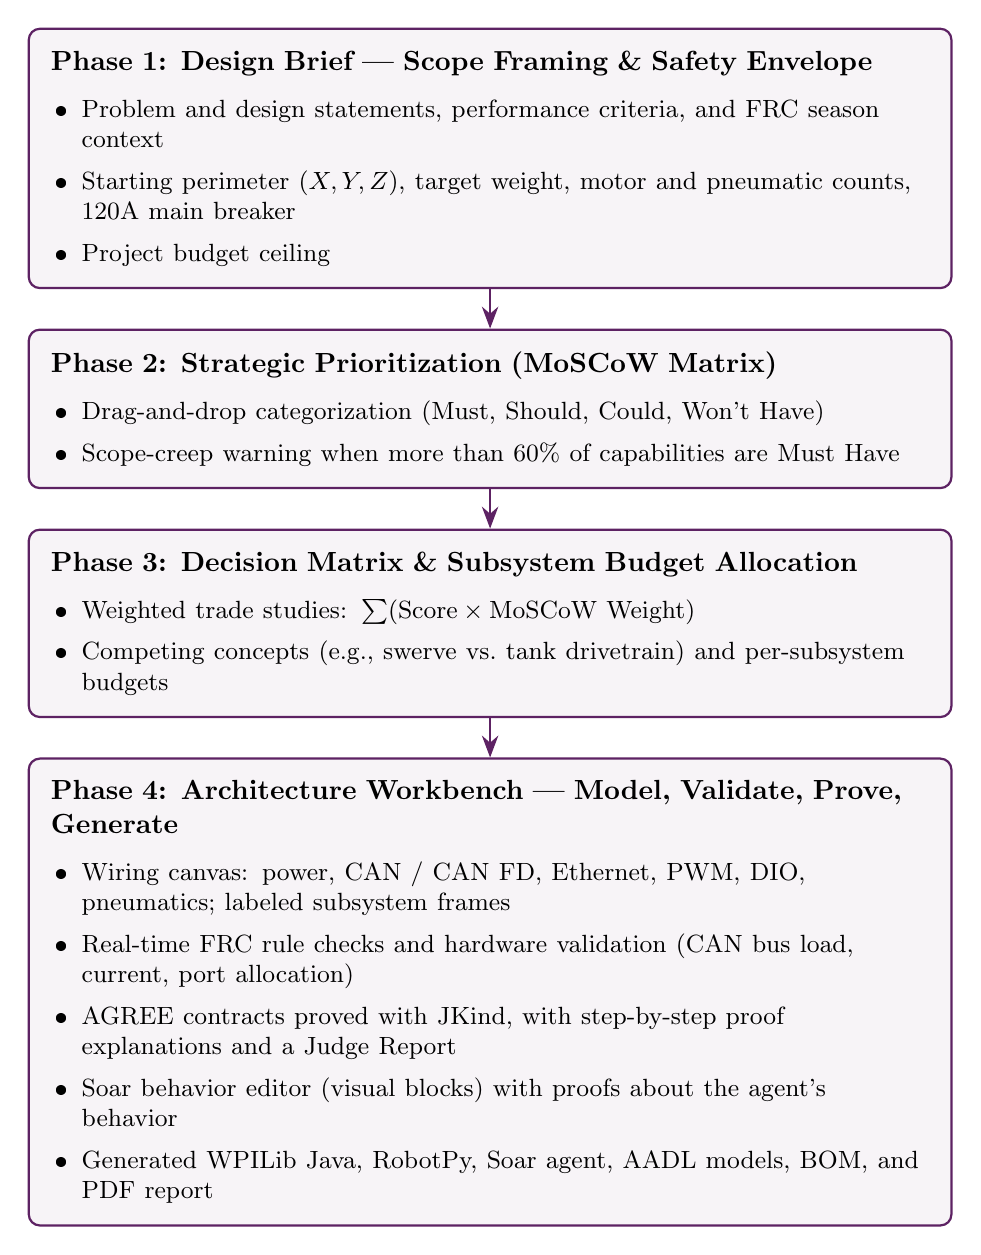
\begin{tikzpicture}[
    node distance=0.5cm,
    block/.style={
        rectangle,
        draw=assistpurple,
        fill=assistpurple!5,
        thick,
        rounded corners=4pt,
        text width=0.92\linewidth,
        inner sep=8pt,
        align=left
    },
    arrow/.style={
        -{Stealth[scale=1.2]},
        thick,
        draw=assistpurple
    }
]

\node (p1) [block] {
    \textbf{{Phase 1: Design Brief --- Scope Framing \& Safety Envelope}}\\
    \small
    \begin{itemize}[leftmargin=1.2em]
        \item Problem and design statements, performance criteria, and FRC season context
        \item Starting perimeter ($X, Y, Z$), target weight, motor and pneumatic counts, 120A main breaker
        \item Project budget ceiling
    \end{itemize}
};

\node (p2) [block, below=of p1] {
    \textbf{{Phase 2: Strategic Prioritization (MoSCoW Matrix)}}\\
    \small
    \begin{itemize}[leftmargin=1.2em]
        \item Drag-and-drop categorization (Must, Should, Could, Won't Have)
        \item Scope-creep warning when more than $60\%$ of capabilities are Must Have
    \end{itemize}
};

\node (p3) [block, below=of p2] {
    \textbf{{Phase 3: Decision Matrix \& Subsystem Budget Allocation}}\\
    \small
    \begin{itemize}[leftmargin=1.2em]
        \item Weighted trade studies: $\sum (\text{Score} \times \text{MoSCoW Weight})$
        \item Competing concepts (e.g., swerve vs.\ tank drivetrain) and per-subsystem budgets
    \end{itemize}
};

\node (p4) [block, below=of p3] {
    \textbf{{Phase 4: Architecture Workbench --- Model, Validate, Prove, Generate}}\\
    \small
    \begin{itemize}[leftmargin=1.2em]
        \item Wiring canvas: power, CAN / CAN FD, Ethernet, PWM, DIO, pneumatics; labeled subsystem frames
        \item Real-time FRC rule checks and hardware validation (CAN bus load, current, port allocation)
        \item AGREE contracts proved with JKind, with step-by-step proof explanations and a Judge Report
        \item Soar behavior editor (visual blocks) with proofs about the agent's behavior
        \item Generated WPILib Java, RobotPy, Soar agent, AADL models, BOM, and PDF report
    \end{itemize}
};

\draw [arrow] (p1) -- (p2);
\draw [arrow] (p2) -- (p3);
\draw [arrow] (p3) -- (p4);

\end{tikzpicture}
\end{center}
\vspace{1em}

\newpage

% ==============================================================================
% SECTION C: DETAILED PHASE CAPABILITIES
% ==============================================================================
\section*{\Large {C. Detailed Phase Capabilities}}\label{sec:C}

\subsection*{\normalsize {C-1 Phase 1: FRC Robot Scope \& Safety Envelope (\texttt{DesignBrief.tsx})}}\label{sec:C1}
The Design Brief introduces students to envelope analysis, a foundational concept in aerospace flight readiness.

\begin{itemize}
    \item \textbf{Problem and Design Statements:} Teams write a formal problem statement, a design statement, and measurable performance criteria.
    \item \textbf{Envelope Bounds:} Starting perimeter ($X, Y, Z$) and a target weight against the FRC limit.
    \item \textbf{Safety \& Compliance Planning:} The required 120A main breaker, planned motor count, and pneumatic count.
    \item \textbf{Cost Constraints:} A project budget ceiling.
\end{itemize}

\subsection*{\normalsize {C-2 Phase 2: Strategic Capability Prioritization (\texttt{Moscow.tsx})}}\label{sec:C2}
Students sort mission requirements on a drag-and-drop board:

\begin{itemize}
    \item \textbf{Categorization Buckets:}
    \begin{itemize}
        \item \textbf{MUST HAVE:} Mission-critical safety and baseline operational features.
        \item \textbf{SHOULD HAVE:} High-value competitive and tactical capabilities.
        \item \textbf{COULD HAVE:} Low-priority stretch capabilities.
        \item \textbf{WON'T HAVE:} Explicitly scoped-out requirements.
    \end{itemize}
    \item \textbf{Scope Guardrails:} A warning appears when more than $60\%$ of capabilities are Must Have, teaching the scope management that defense and aerospace programs depend on.
\end{itemize}

\subsection*{\normalsize {C-3 Phase 3: Multi-Criteria Trade Studies (\texttt{Brainstorming.tsx})}}\label{sec:C3}
Trade studies turn qualitative strategy discussions into quantified engineering decisions:

\begin{equation}
\text{Weighted Score} = \sum_{i=1}^{n} \left( \text{Score}_i \times \text{Weight}_i(\text{MoSCoW}) \right)
\end{equation}

\begin{itemize}
    \item \textbf{MoSCoW Weight Mapping:} MUST HAVE ($w=3$), SHOULD HAVE ($w=2$), COULD HAVE ($w=1$), carried over automatically from Phase 2.
    \item \textbf{Concept Scoring:} Competing physical or software design options are scored against every weighted criterion.
    \item \textbf{Subsystem Cost Decomposition:} Spending ceilings for individual subsystems (e.g., drivetrain, intake, vision, manipulators).
\end{itemize}

\needspace{6cm}
\subsection*{\normalsize {C-4 Phase 4: Architecture Workbench \& Hardware Validation (\texttt{ArchitectureCanvas.tsx})}}\label{sec:C4}
The architecture workbench is laid out like a professional engineering IDE: an activity bar for components, contracts, behavior, and exports; editor tabs for the diagram, contracts, generated files, and the behavior editor; and a bottom panel for problems, hardware analysis, and proofs. The wiring canvas is built on \texttt{@xyflow/react}.

\begin{itemize}
    \item \textbf{Component Catalog:}
    \begin{itemize}
        \item \textbf{Robot Controllers:} SystemCore (default, for the 2027 season and later) and the NI roboRIO 2.0 (2026 and earlier), each with its own port map.
        \item \textbf{Power \& Communication:} Battery, 120A main breaker, REV PDH, voltage regulators and buck converters, VH-109 radio, RSL, CTRE CANivore, CAN hubs, Ethernet switches.
        \item \textbf{Actuators:} Kraken X60/X44, Falcon 500, NEO, NEO Vortex, NEO 550, brushed motors, servos, and REV pneumatics.
        \item \textbf{Sensors \& Vision:} CANcoder, Pigeon 2.0 IMU, through-bore encoders, limit switches, beam breaks, LaserCAN, color sensors, Limelight, PhotonVision cameras, and Linux coprocessors.
        \item \textbf{Wire Types:} Battery, 40A and 15A PDH channels, regulated power, CAN (1 Mbps), CAN FD (8 Mbps), Ethernet, PWM, DIO, RSL, USB, and pneumatic lines, each drawn in its own style. Wires of the wrong type cannot be connected.
    \end{itemize}
    \item \textbf{Subsystems:} Devices are grouped into labeled subsystem frames (for example, ``Intake''). The frames carry through to generated code and to the robot's behavior.
    \item \textbf{Real-Time FRC Rule Checks (\texttt{systemVerifier.ts}):} Battery-to-breaker-to-PDH power chain, one robot controller, RSL wiring, CAN bus origin and 120$\Omega$ termination, CAN chain continuity, motors on correctly sized PDH channels, unregulated coprocessor power, pneumatics wiring, controller port limits, and controller-specific rules such as the absence of an MXP port on SystemCore. A compliance score ($0$--$100\%$) summarizes the result.
    \item \textbf{Hardware Validation (\texttt{hardwareValidation.ts}):} Estimated CAN bus load for each bus, current roll-up for each PDH channel, regulator, and the main breaker, duplicate or out-of-range CAN IDs, and DIO, PWM, and Smart I/O allocation. Every estimate is a named, documented constant, so students can see where each number comes from.
\end{itemize}

\newpage

% ==============================================================================
% SECTION D: FORMAL VERIFICATION
% ==============================================================================
\section*{\Large {D. Formal Verification with AADL, AGREE \& JKind}}\label{sec:D}
SysMod Studio teaches compositional formal verification, the approach used for safety-critical avionics architectures \cite{agree}. Each wiring diagram becomes an \textbf{AADL} model \cite{aadl}, and each device type carries an \textbf{AGREE} contract: \emph{assumptions} about its inputs and \emph{guarantees} about its outputs.

\begin{itemize}
    \item \textbf{Standard FRC Contracts:} SysMod provides contracts for common devices (for example, the voltage range a motor controller needs and the current a PDH channel can supply). Students add their own assumptions, guarantees, and system-level lemmas in a code editor with AGREE syntax highlighting and error checking.
    \item \textbf{Local Proofs without OSATE:} SysMod translates the contracts to Lustre and runs the \textbf{JKind} model checker \cite{jkind} on the student's computer, with a bundled Java runtime. Students do not install Java, Eclipse, or OSATE.
    \item \textbf{Counterexamples:} When a property fails, JKind returns a concrete trace that shows the inputs that break it.
    \item \textbf{Explained Proofs:} Using JKind's inductive validity cores (the facts each proof actually needed), SysMod writes each proof as a two-column, step-by-step argument: which wires and which guarantees imply the property.
    \item \textbf{Judge Report:} A printable report presents every proof for FRC judges, award reviewers, and mentors who do not know AADL.
\end{itemize}

This mirrors the workflow aerospace engineers use to build architecture-level safety evidence: model the system, state contracts, prove them with a model checker, and present the evidence to reviewers.

\needspace{8cm}
% ==============================================================================
% SECTION E: ROBOT BEHAVIOR (SOAR)
% ==============================================================================
\section*{\Large {E. Robot Behavior: Soar Agents \& Verified Autonomy}}\label{sec:E}
Autonomous aircraft must make decisions that can be explained and checked. SysMod Studio introduces this idea through the robot's own decision-making, using \textbf{Soar} \cite{soar}, a cognitive architecture from the University of Michigan that has been used for decades in robotics and in models of human operators and pilots.

\subsection*{\normalsize {E-1 Building an Agent with Blocks}}\label{sec:E1}
\begin{itemize}
    \item \textbf{Visual Rules:} Students build the agent from Blockly blocks: \emph{operators} proposed when sensor conditions hold, \emph{apply} rules that command devices, and \emph{elaborations}. Priorities (best, worst, required) decide between operators.
    \item \textbf{Connected to the Diagram:} The blocks read sensors and command the devices and subsystem frames on the student's architecture diagram.
    \item \textbf{Real Soar Output:} The blocks generate a Soar 9.6.5 agent (\texttt{agent.soar}). The generated robot code connects it to the robot through the FRC-Soar bridge, which sends sensor readings and the match mode to the agent each loop and carries out the commands it returns.
\end{itemize}

\subsection*{\normalsize {E-2 Proving Facts About the Agent}}\label{sec:E2}
Building on recent Florida Tech research that translates Soar models into model checkers \cite{soar2prism}, SysMod Studio lets students prove facts about their agent's behavior, not just test it:

\begin{itemize}
    \item \textbf{Property Templates:} ``\emph{A command is only sent in a given robot mode},'' ``\emph{two devices are never in these states at the same time},'' and ``\emph{can the agent ever send this command?}'' Students fill these in from dropdowns.
    \item \textbf{Every Possible Match:} The agent becomes an AADL \texttt{Soar\_Agent} component with a generated AGREE contract, in which one step is one robot loop. Sensor readings are encoded exactly relative to the values the rules test, and ties between equal operators are left to an unconstrained choice. A proof therefore covers every sensor reading, every choice Soar can make, and matches of any length.
    \item \textbf{Counterexamples in Plain Words:} When a property fails, SysMod shows the match loop by loop: the robot mode, each sensor reading, what Soar chose, and what the robot was sent.
    \item \textbf{A Validated Model:} A proof is only as good as the model it is about. SysMod's model of the agent was checked loop by loop against real Soar 9.6.5 on 1,016 randomly generated programs (121,920 robot loops) with no disagreements, and the AGREE translation was checked against that model on hundreds more.
\end{itemize}

\newpage

% ==============================================================================
% SECTION F: CODE GENERATION & EXPORTS
% ==============================================================================
\section*{\Large {F. Code Generation \& Exports}}\label{sec:F}
SysMod Studio connects high school robotics practice with professional engineering artifacts:

\vspace{0.8em}
\needspace{8cm}
\begin{cardtable}{>{\bfseries\color{assistpurple}}L{3.0cm} L{3.2cm} Y}{SysMod Studio Outputs and Workforce Skill Connections}
\rowcolor{tableheader}
\color{white}\bfseries Target Domain & \color{white}\bfseries Language / Spec & \color{white}\bfseries Workforce Skill \& Aerospace Connection \\
\rowcolor{white}
Embedded Robot Software & WPILib Java and RobotPy (Python) & Command-based subsystem classes with CAN IDs, ports, and current limits from the diagram, the starting point for a team's robot code. Teaches structured embedded control software. \\
\hline
\rowcolor{tablealt}
Autonomous Decision-Making & Soar agent (\texttt{agent.soar}) & A rule-based cognitive agent, plus the robot code that connects it to sensors and actuators. Introduces explainable, symbolic autonomy. \\
\hline
\rowcolor{white}
Architecture Models & AADL (SAE AS5506) with AGREE contracts & The robot architecture and the Soar agent as AADL models, introducing the architecture language used in avionics and aerospace system analysis. \\
\hline
\rowcolor{tablealt}
Formal Evidence & Lustre / JKind proofs and the Judge Report & Machine-checked proofs and counterexamples, explained step by step: practice in building and presenting safety evidence. \\
\hline
\rowcolor{white}
Engineering Documentation & HTML / PDF report & Schematic, bill of materials (BOM), and system specification, teaching rigorous engineering documentation. \\
\end{cardtable}

\needspace{6cm}
% ==============================================================================
% SECTION G: ALIGNMENT WITH NASA ULI TRANSCEND FRAMEWORK
% ==============================================================================
\section*{\Large {G. Alignment with NASA ULI TRANSCEND Framework}}\label{sec:G}

SysMod Studio aligns with the four core pillars, technical challenge thrusts (TC1--TC4), and high-level assurance goals of the NASA ULI TRANSCEND framework:

\vspace{0.8em}
\begin{cardtable}{>{\bfseries\color{assistpurple}}L{3.2cm} L{3.2cm} Y}{Mapping SysMod Studio to TRANSCEND Core Pillars and Technical Challenges}
\rowcolor{tableheader}
\color{white}\bfseries TRANSCEND Pillar & \color{white}\bfseries Technical Thrust (TC) & \color{white}\bfseries SysMod Studio Implementation \\
\rowcolor{white}
Human-Computer Interaction & TC1: Trustworthiness Models \& Measures & An engineering workbench designed for students: visual wiring, real-time rule and hardware feedback, and verification results in plain language. \\
\hline
\rowcolor{tablealt}
Explainable AI & TC2: Assured Autonomy Design Methods \& Tools & Transparent decision matrices; a symbolic Soar agent whose rules students can read; step-by-step proof explanations and counterexamples told loop by loop. \\
\hline
\rowcolor{white}
ML-based Analyses & TC3: Integration, Simulation \& Evaluation Framework & Modeling of vision coprocessors (Limelight, PhotonVision) and their power and network integration; a reference simulator of the Soar agent, validated against real Soar. \\
\hline
\rowcolor{tablealt}
Formal Methods & TC4: Evaluation \& Safety Case Methodology & AADL models with AGREE contracts proved by JKind, for both the electrical architecture and the autonomous agent; a Judge Report that presents the evidence. \\
\end{cardtable}

\vspace{0.8em}
\begin{cardtable}{>{\bfseries\color{assistpurple}}L{2.8cm} Y}{SysMod Studio Support for TRANSCEND Core Assurance Goals}
\rowcolor{tableheader}
\color{white}\bfseries Assurance Goal & \color{white}\bfseries Operational Delivery in SysMod Studio \\
\rowcolor{white}
TRUSTWORTHY & Real-time checks of breaker placement, power channels, CAN topology, and bus load; machine-checked proofs of device contracts and of the agent's behavior, over every possible input. \\
\hline
\rowcolor{tablealt}
BELIEVED & Transparent trade studies, a clear visual architecture, and proofs explained step by step, so mentors and judges can see why a property holds or how it fails. \\
\hline
\rowcolor{white}
RELIED UPON & Generated robot code, Soar agent, BOM, and engineering reports that teams use directly in their build season. \\
\end{cardtable}

\needspace{6cm}
% ==============================================================================
% SECTION H: TECHNICAL IMPLEMENTATION & QUALITY ASSURANCE
% ==============================================================================
\section*{\Large {H. Technical Implementation \& Quality Assurance}}\label{sec:H}
\begin{itemize}
    \item \textbf{Desktop Application:} Electron with electron-vite; free installers for Windows and Linux, published as GitHub releases. Documentation is hosted on Read the Docs.
    \item \textbf{Frontend:} React 19, TypeScript, Tailwind CSS 4 with daisyUI, and \texttt{lucide-react} icons.
    \item \textbf{Graph Engine:} \texttt{@xyflow/react} (React Flow v12) with custom node types for controllers, devices, and subsystem frames.
    \item \textbf{Editors:} Monaco (the editor behind VS Code) with AADL, AGREE, and Soar highlighting; Blockly 13 for behavior blocks.
    \item \textbf{State Management \& Interaction:} Zustand; \texttt{@hello-pangea/dnd} for drag-and-drop prioritization.
    \item \textbf{Verification:} An AGREE parser and Lustre generator written for SysMod; the JKind model checker with a trimmed, bundled Java runtime.
    \item \textbf{Document Synthesis:} HTML-to-PDF preview for the specification report, and a printable Judge Report.
    \item \textbf{Continuous Integration:} Every change is built and tested on Windows and Linux: hardware-rule checks, proofs of the standard FRC contracts with JKind, and behavior checks that load every generated agent into real Soar 9.6.5 and compare it, loop by loop, with SysMod's model.
\end{itemize}

\needspace{8cm}
% ==============================================================================
% SECTION I: STRATEGIC WORKFORCE PIPELINE
% ==============================================================================
\section*{\Large {I. Strategic Workforce Pipeline: FIRST to Autonomous Aviation}}\label{sec:I}

\subsection*{\normalsize {I-1 Educational Progression \& Skill Mapping}}\label{sec:I1}
SysMod Studio establishes an educational pipeline that links K-12 robotics with the aerospace industry's future needs:

\vspace{0.8em}
\begin{cardtable}{>{\bfseries\color{assistpurple}}L{3.0cm} L{3.5cm} Y}{The FIRST-to-Aerospace Talent Pipeline Skill Matrix}
\rowcolor{tableheader}
\color{white}\bfseries Pipeline Stage & \color{white}\bfseries Applied Tool Environment & \color{white}\bfseries Acquired Industry Competency \\
\rowcolor{white}
High School (FRC Teams) & SysMod Studio & MBSE principles, bus topology design, trade studies, contract-based verification, rule-based autonomy, and robot code generation. \\
\hline
\rowcolor{tablealt}
University / Research (Florida Tech / NASA ULI) & ASSIST Lab; SysMod Studio with the full AADL toolchain (OSATE, AGREE) & Formal safety verification, model checking of cognitive and autonomous agents, and safety-critical architecture design. \\
\hline
\rowcolor{white}
Industry Workforce (NASA, Aerospace, AAM) & Enterprise MBSE and verification tools & Systems engineers proficient in MBSE, airworthiness evidence, autonomous system integration, and safety assurance. \\
\end{cardtable}
\vspace{0.8em}

\subsection*{\normalsize {I-2 Feasibility, Feeder Pipeline \& Return on Investment}}\label{sec:I2}
By introducing FRC students to systems thinking early, SysMod Studio demystifies MBSE and formal methods. Students who use it arrive at university aerospace programs with practical experience in CAN bus topologies, rule checking, trade studies, AADL modeling, contract-based proofs, and verified autonomous behavior. Because the tool is free, runs on ordinary school laptops, and fits into the build season teams already have, it can reach teams without new budget or staff. This offers NASA and commercial aviation partners an early, low-cost path to job-ready talent in autonomous systems.

\needspace{6cm}
% ==============================================================================
% SECTION J: CURRENT STATUS, LIMITATIONS & ROADMAP
% ==============================================================================
\section*{\Large {J. Current Status, Limitations \& Roadmap}}\label{sec:J}

\vspace{0.4em}
\begin{cardtable}{>{\bfseries\color{assistpurple}}L{3.0cm} Y}{Status of SysMod Studio, November 2026}
\rowcolor{tableheader}
\color{white}\bfseries Area & \color{white}\bfseries Status \\
\rowcolor{white}
Available now & Planning phases; architecture workbench with FRC rule checks and hardware validation; AGREE contracts proved with JKind and the Judge Report; Soar behavior editor; proofs about the agent's behavior; Java, Python, Soar, and AADL generation; Windows and Linux releases. \\
\hline
\rowcolor{tablealt}
Known limitations & Projects are not yet saved to disk automatically. Generated robot code has not yet been compiled against the real WPILib and vendor libraries. The generated AADL has not yet been checked in OSATE. Behavior proofs consider every reading a sensor could send, including values a given sensor never produces. SystemCore power and brownout figures are left out until they are published. \\
\hline
\rowcolor{white}
Next steps & Pilot use with FRC teams; saving projects; SystemCore rules and WPILib 2027 code after the 2027 FRC kickoff (January 9, 2027); running Soar agents on the robot through the FRC-Soar bridge; response-time properties (``within $N$ loops''); probabilistic analysis of agent behavior with PRISM, following \cite{soar2prism}. \\
\end{cardtable}

\needspace{4cm}
% ==============================================================================
% SECTION K: CONCLUSION
% ==============================================================================
\section*{\Large {K. Conclusion}}\label{sec:K}
SysMod Studio is a free, accessible, and mathematically grounded workforce development platform. Developed by Alexander Doyle and team in the ASSIST Laboratory at Florida Tech under NASA ULI TRANSCEND, it turns FIRST Robotics experience into early practice with the methods the future aerospace workforce will use: model-based systems engineering, contract-based formal verification, and autonomous decision-making that can be explained and proved. The result is a feeder pipeline toward the engineers who will build the next generation of trustworthy autonomous aviation systems.

% ==============================================================================
% REFERENCES
% ==============================================================================
\phantomsection\label{sec:refs}
\renewcommand{\refname}{\Large References}
\begin{thebibliography}{9}
\small
\bibitem{aadl} SAE International. \emph{Architecture Analysis \& Design Language (AADL)}, SAE Standard AS5506.

\bibitem{agree} D.~Cofer, A.~Gacek, S.~Miller, M.~W.~Whalen, B.~LaValley, and L.~Sha. Compositional verification of architectural models. In \emph{NASA Formal Methods (NFM)}, 2012.

\bibitem{jkind} A.~Gacek, J.~Backes, M.~W.~Whalen, L.~Wagner, and E.~Ghassabani. The JKind model checker. In \emph{Computer Aided Verification (CAV)}, 2018.

\bibitem{soar} J.~E.~Laird. \emph{The Soar Cognitive Architecture}. MIT Press, 2012.

\bibitem{soar2prism} P.~Ganeriwala, C.~Chambers, J.~I.~Lathrop, S.~Bhattacharyya, J.~Babar, S.~B.~Gilbert, I.~Amundson, M.~C.~Dorneich, and M.~A.~H.~Khan. Formal analysis of stochastic cognitive models: A translation framework from Soar to PRISM. In \emph{NASA Formal Methods (NFM)}, 2026.
\end{thebibliography}

\end{document}
